\chapter{Fitting of Spectra}
\label{appendix:fitting}

The spectra of Ba\textsuperscript{+} deposits in SXe are described in detail for green excitation ($\sim$540-590~nm) in Sec. \ref{sec:fluorescence}, and for blue excitation ($\sim$460-490~nm) in Sec. \ref{sec:BaPlus}.  Chi-square fitting to these spectra using ROOT is described in this section.  In most circumstances, the different fluorescence peaks in a spectrum overlap somewhat.  Thus it was necessary to fit the fluorescence spectra with a sum of peak-specific fit functions in order to extract peak heights and integrals.  These were used, e.g., in excitation spectra, annealing, and bleaching curves for different peaks.  Gaussians, Lorentzians and asymmetric functions were used, depending on the best match to a specific peak.  When extracting fluorescence peak amplitudes from spectra, shape parameters (center and widths) were fixed, and amplitudes were allowed to float.  Determination of those fixed shape parameters was done prior, by fitting spectra where the peak of interest is strong and letting all parameters float.

%The center and width parameters of the fit functions were fixed, while the amplitudes were the free fitting parameters.  Center and width parameters for each peak were determined by fitting spectra where that peak is relatively large.  Some fine-tuning was done to match slightly different shapes resulting from different excitation wavelengths.

\section{Fitting Spectra with Green Excitation}
\label{sec:fitgrn}

\begin{figure} %[H]
        \centering
                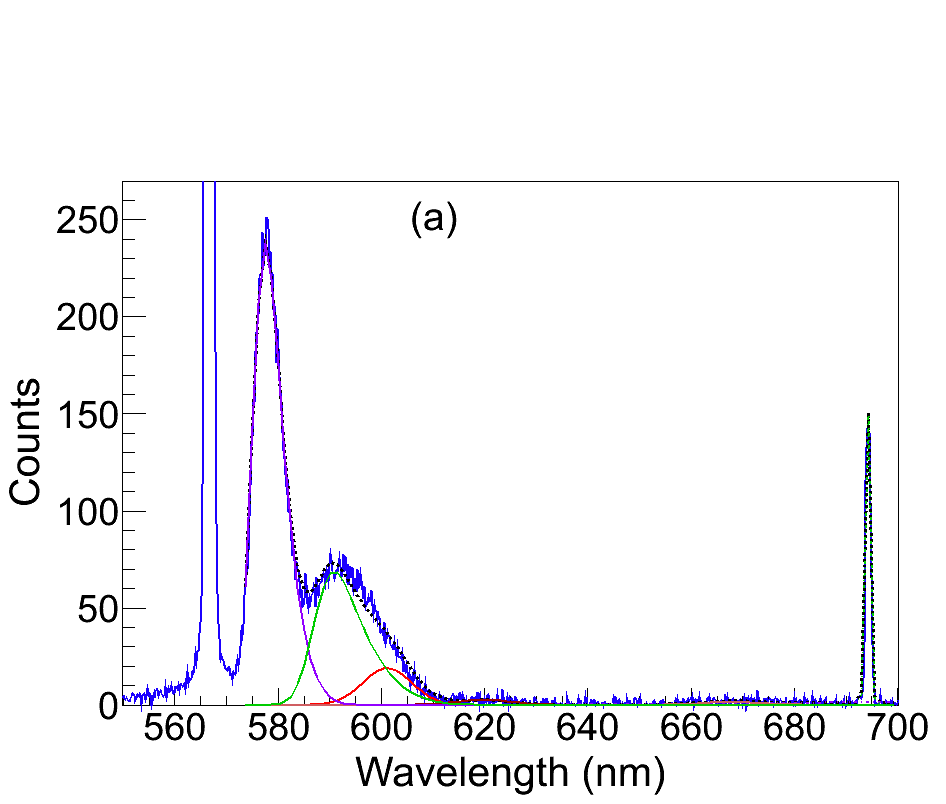
\includegraphics[width=.5\textwidth]{figures/spectra_fit_a.png}
                ~
                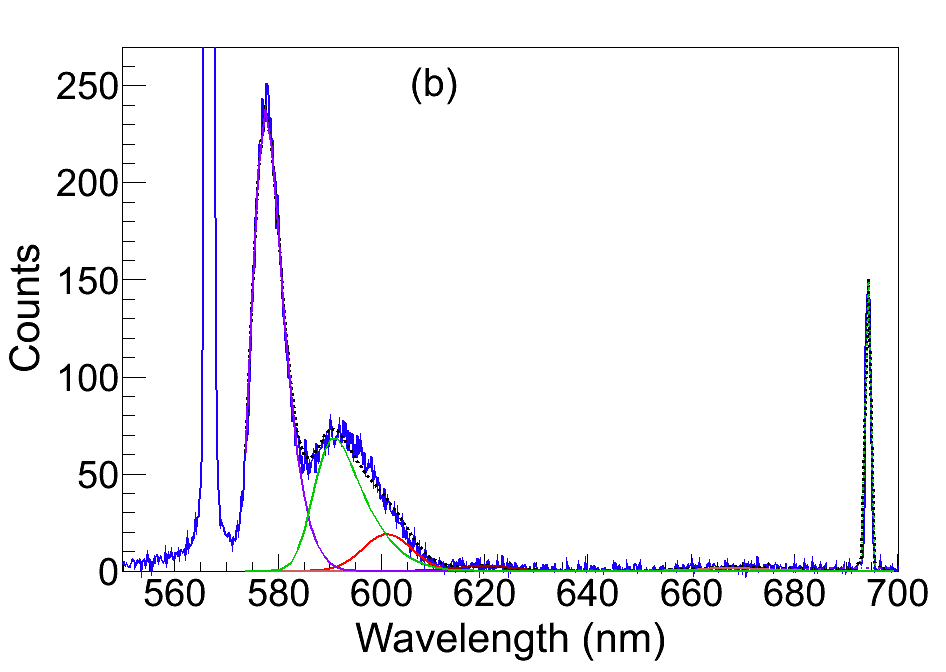
\includegraphics[width=.5\textwidth]{figures/spectra_fit_b.png}
                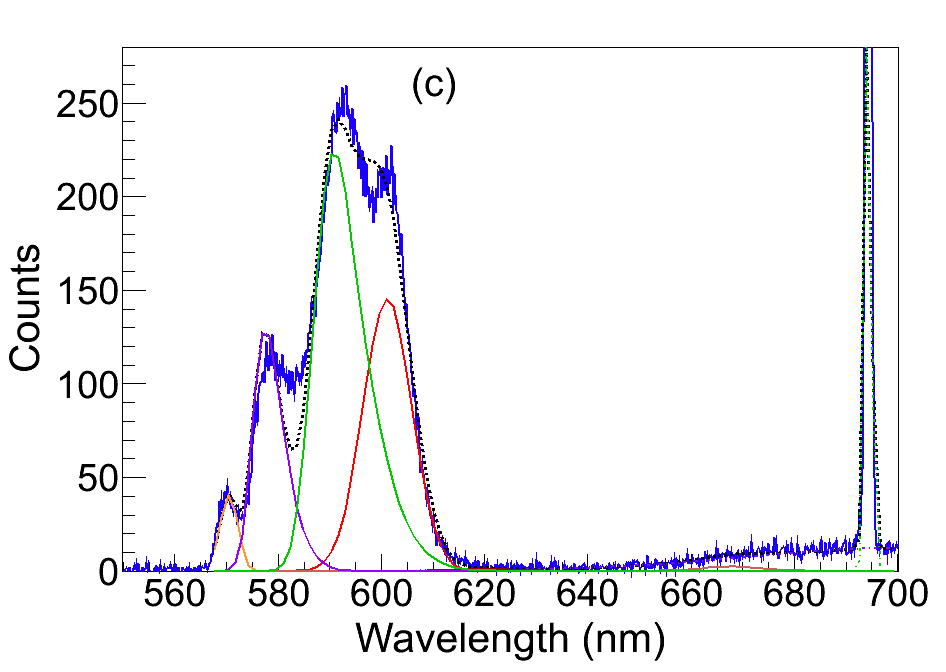
\includegraphics[width=.5\textwidth]{figures/spectra_fit_c.png}
                ~
                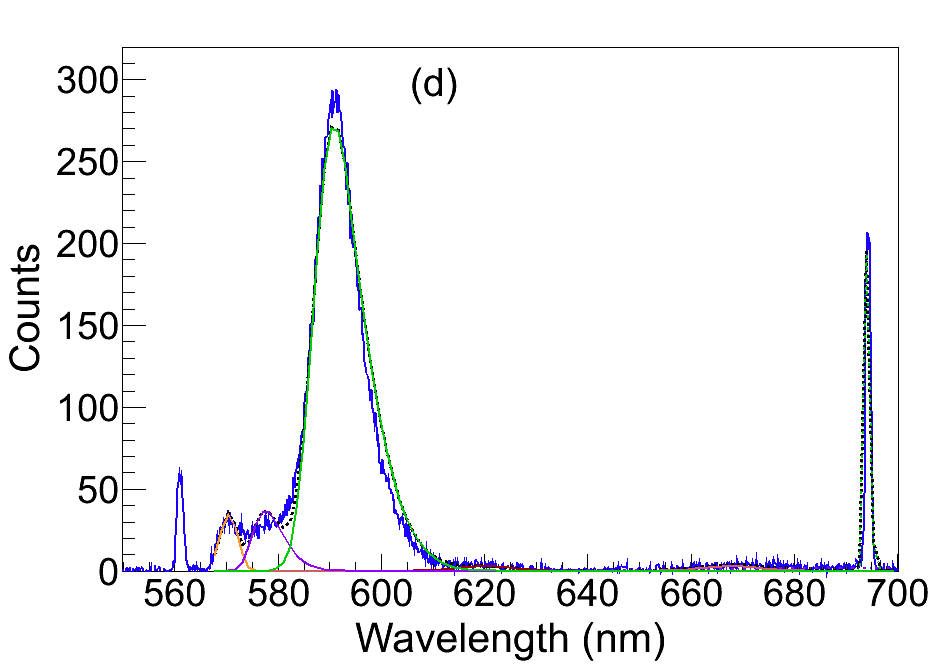
\includegraphics[width=.5\textwidth]{figures/spectra_fit_d.png}
                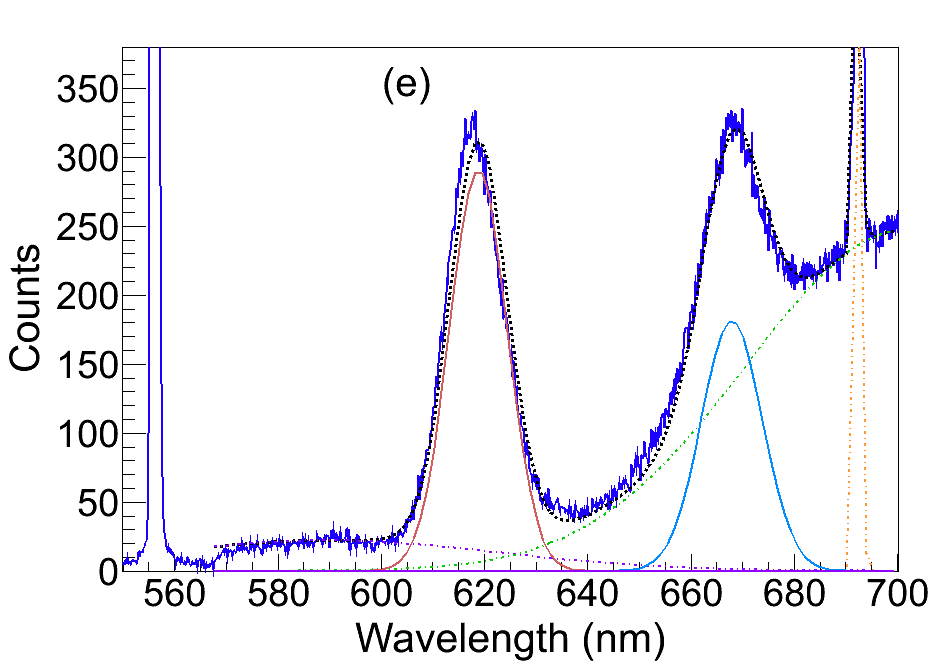
\includegraphics[width=.5\textwidth]{figures/spectra_fit_e.png}
                ~
                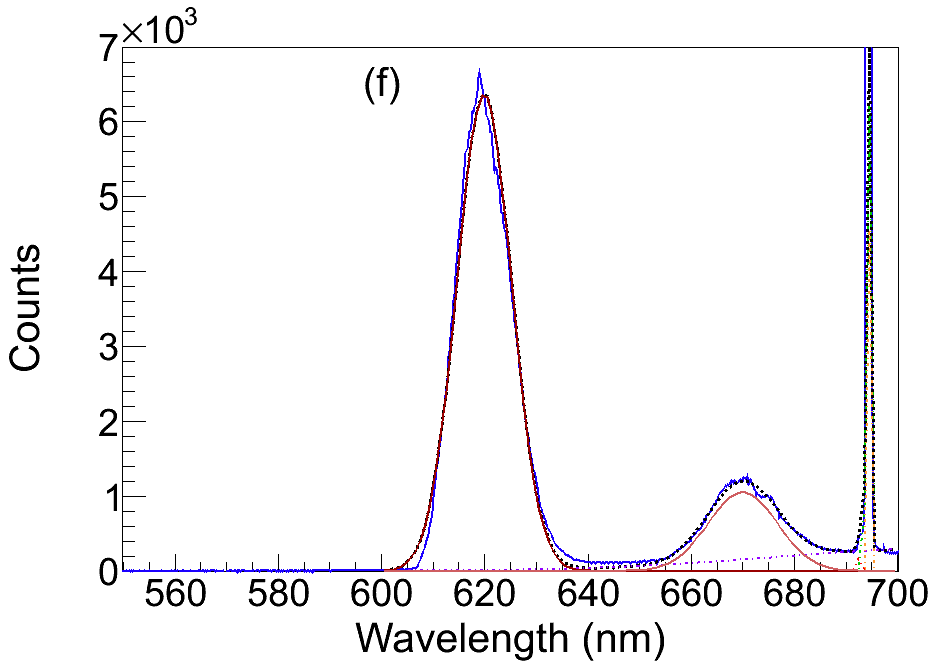
\includegraphics[width=.5\textwidth]{figures/spectra_fit_f.png}
                \caption{Example fits to spectra of Ba\textsuperscript{+} deposits with green excitation at (a) 567.3~nm, (b) 566.6~nm, (c) 563.4~nm, (d) 561.0~nm, (e) 555.9~nm, and (f) 546.3~nm.  Laser scatter can be seen in the lower wavelengths for some figures, especially in (b) where it is on the edge of the Raman filter cutoff.}
\label{fig:specFitsGrn}
\end{figure}

Example fits to spectra for several different green excitation wavelengths are shown in Fig. \ref{fig:specFitsGrn}.  To incorporate the tail in the shape of the 577- and 591-nm peaks, an asymmetric function of the form $A(1+$erf$(\frac{x-a}{\sigma_{1}})(1-$erf$(\frac{x-a}{\sigma_{2}}))$ was used, where $a$ is the fixed center-defining parameter, $\sigma_{1}$ and $\sigma_{2}$ are fixed left and right width parameters, and $A$ is the free amplitude parameter.  The function erf() is an error function.  The 570-, 601-, 619-, and 670-nm peaks were fit with Gaussian functions with fixed standard deviation ($\sigma$) of 1.7~nm, 4.7~nm, 5.3~nm, and 6.7~nm, respectively.  Rather than attempting frame-by-frame background subtractions, additional Gaussians were fit to the broad and sharp background fluorescence.  Two broad Gaussians centered at around 590~nm and 702~nm, and one sharp Gaussian near 693~nm, were chosen by fitting spectra of Xe-only deposits.  These backgrounds and their excitation spectra are discussed in Appendix \ref{appendix:bgs}.  The full fit, i.e. the sum of each contributing peak fit, is the dotted black line.  Though the shapes do not match perfectly for all excitation wavelengths, the fits still follow the peak amplitudes well.  Ba emission and excitation spectra results are discussed in Sec. \ref{sec:fluorescence}.

\section{Fitting Spectra with Blue Excitation}
\label{sec:fitblu}

Example fits to spectra for several different blue excitation wavelengths are shown in Fig. \ref{fig:specFitsBlu}.  Gaussian functions were used for the 532-, 568-, and 575-nm peaks with standard deviations ($\sigma$) of 2.4~nm, 5.0~nm, and 0.7~nm, respectively.  Lorentzian functions were used for the 553-, 592-, 635-, and 669-nm peaks with half width at half maxima ($\gamma$) of 1.7~nm, 13.8~nm, 10.4~nm. and 9.1~nm, respectively.  Similar to spectra with green excitation, the background components were fit with two broad Gaussians centered at 546.0~nm and 703.3~nm, with respective $\sigma$ of 49.0~nm and 30.5~nm, as well as one sharp Gaussian centered at 693.4~nm peak with a $\sigma$ of 0.5~nm.  The fits for excitation around 478~nm (e.g., (c)) are not quite right, mainly due to a shift in the central value of the 592-nm peak.  However, fit values still follow respective peaks heights well.  The sharp 522- and 575-nm peaks are seen in (c), though the 522-nm peak is left out of the fitting range since it sits on the edge of the Raman filter cutoff.   These spectra are discussed in Sec. \ref{sec:BaPlus}.

\begin{figure} %[H]
        \centering
                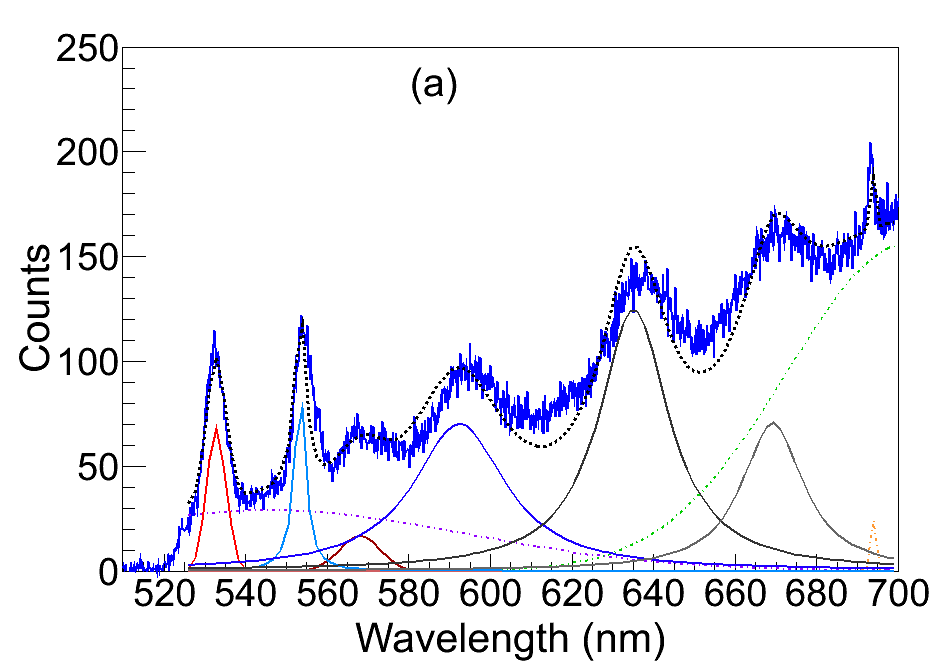
\includegraphics[width=.5\textwidth]{figures/spectra_blu_fit_a.png}
                ~
                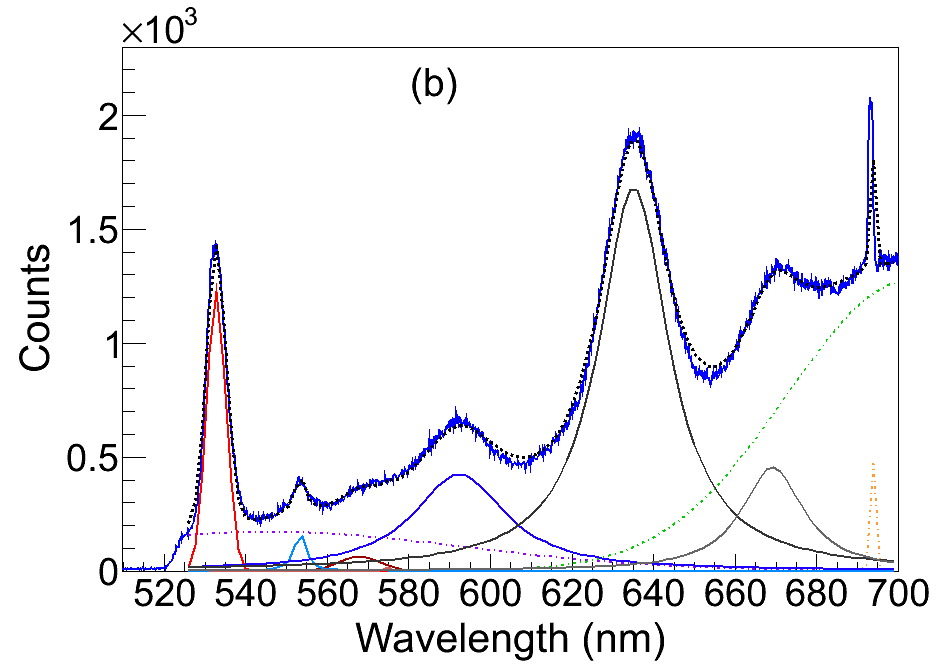
\includegraphics[width=.5\textwidth]{figures/spectra_blu_fit_b.png}
                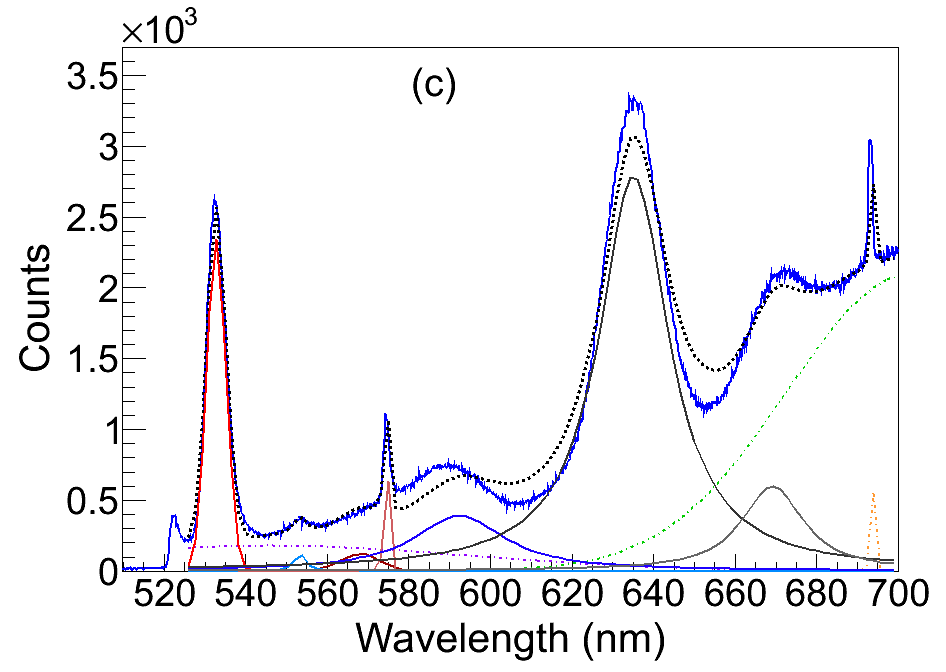
\includegraphics[width=.5\textwidth]{figures/spectra_blu_fit_c.png}
                ~
                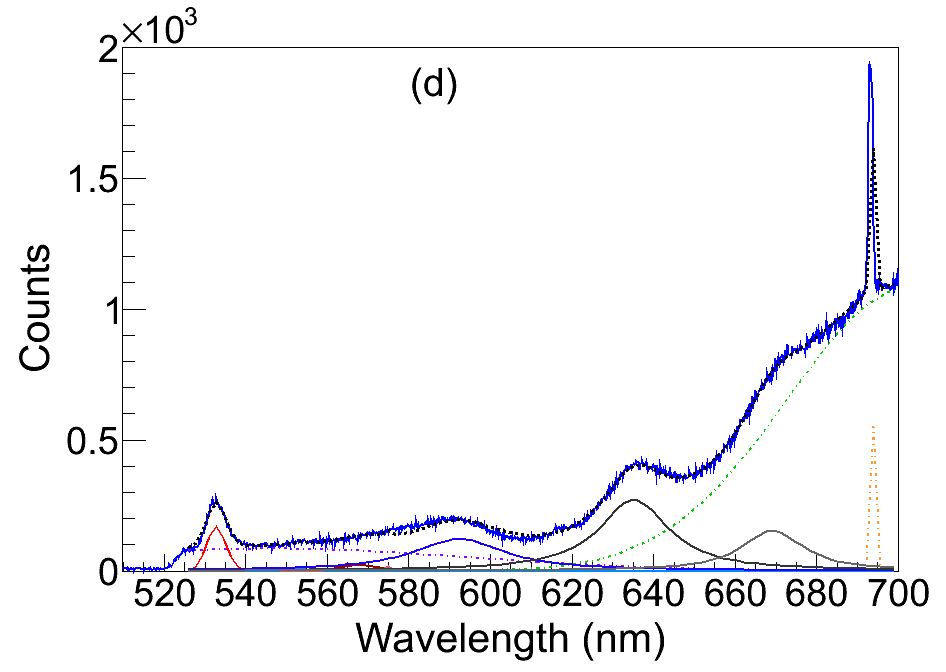
\includegraphics[width=.5\textwidth]{figures/spectra_blu_fit_d.png}
                \caption{Example fits to spectra of Ba\textsuperscript{+} deposits with blue excitation at (a) 461.7~nm, (b) 468.2~nm, (c) 478.3~nm, and (d) 488.2~nm.}
\label{fig:specFitsBlu}
\end{figure}